\chapter{Literature Review}
\label{ch:lit}

\section{Impact of Urban Noise on Health and Wellbeing}

\cit{Environmental noise in Europe 2020}

\hl{Give a full formal background to why noise control is important for public health}.
% https://www.euro.who.int/__data/assets/pdf_file/0008/383921/noise-guidelines-eng.pdf?ua=1

\section{Current Methods of Assessing and Addressing Urban Noise}

The approach to a practical predictive soundscape model arrived at within this thesis is heavily based on past environmental acoustics approaches. I will therefore begin with a brief summary of these past approaches.

\subsection{Acoustical Parameters}

\subsection{ISO Environmental Acoustics Standards}
\hl{ISO 1996-1, esp sections on annoyance, e.g. Annex F, G, H}

\subsection{EU Noise Mapping}

\cit{Environmental noise in Europe 2020}

\subsection{Shortcomings}


\section{Soundscape Studies}

\subsection{Soundscape Descriptors and Indices}

\subsection{Soundwalks}
%TODO: Lit review of the concept of soundwalks
%FIXME: This section on collective soundscapes belongs somewhere else.
Soundwalks, following \gls{wsp} have focussed on the soundscape as 1) an individual's experience of a particular space or 2) as the sonic expression of a culture or community's relationship with the space \citep{Droumeva2021sound}. Starting with Schafer's framing of the soundscape as a collective composition balancing background and foreground sounds, soundmarks and primary sound types, to the \gls{iso} definition of a soundscape, the totality of the acoustic and contextual environment is processed and interpreted by an individual. Despite the \gls{iso}'s expansion from the individual to a group highlighted by the phrasing "by a person, or people", the tools it presents -- and, in particular, how they have been employed -- fail when attempting to address the perception of many people.

This conceptual difficulty in dealing with the perception of many people has contributed to the problems associated with incorporating perception-focussed approaches in practice and regulation. \draft{Read and integrate some section on the purpose of regulation. Peter John 2011 'Making Policy Work'} %TODO: Policy discussion

\subsection{Swedish Soundscape Quality Protocol}


\subsection{Demographic differences}
Several studies have attempted to study the degree to which personal and demographic factors influence a person's soundscape perception. In some conceptions \cit{Kou2020effects} % CITE add Erfanian 2020
these personal factors are classed as 'contextual' soundscape indicators - features which influence or, in a modelling context, be used as independent variables to predict the value of a soundscape descriptor. The personal factors help to create a personal soundscape interpretation model which is individual to each person.

In this way, a person's individual state-of-mind, ethnic identity, educational background, gender identity, etc. form a pseudo-deterministic framework %! what a load of crap
through which the physical inputs from their environment are filtered. Clearly, many of these personal factors could never be measured and even those which are measurable will have wide ranges of legitimate effects, however estimating the degree and type of effect they may have can both help us better predict individual soundscape assessments and understand how group identities influence sound perception.

%TODO: Need to include earlier, more foundational studies into demographic factors

\paragraph*{Section on Erfanian et al. 2020, Psychological Well-being}

\paragraph*{Low-income and minority evidence} % FIXME I think this section will need to be heavily revised for phrasing and content. I'm not happy with how I'm discussing under-represented groups.
A consistent limitation of soundscape studies investigating the influence of personal factors is a sampling bias towards majority ethnicities (typically White British for UK studies and ethnic Chinese for Chinese studies) and middle-class and highly educated groups. % CITE Hoo boy citation definitely needed
This results in not only incomplete information about how demographics influence soundscape perception, but also represents a systemic under-representation of certain environments. While it may be unclear to what extent ethnicity and social class internally influence a person's perception, it is clear that these groups are exposed to different sound environments % NOTE: socio-economic studies - Huan 2019? Jian ~2015?, Environmental noise in Europe 2020

and therefore studies which do not include under-represented groups are also by definition not including those sound environments which those groups inhabit.

A recent study by \cit{Kou2020effects} was successful in making inroads in these under-represented environments by studying the Humboldt Park neighbourhood in Chicago, USA. Their study included
% TODO: Finish summarising results from Kou2020


\section{Approaches to Soundscape in Engineering}

From this literature review, some conclusions about current approaches to incorporating the concept of "soundscape" into practical engineering and architectural design have been identified.

\subsection{The Quiet Areas approach}

This approach maintains a focus on "identifying and preserving quiet areas" \citep{EEA2020Environment} following the imperative given in the \gls{end} \citep{EU2002Directive}. This approach is mostly rooted in a noise mindset, although the methods employed for identifying quiet areas vary across countries within the EEA. Background sound levels seem to play an important role in identifying quiet areas, in particular when attempting to produce maps of available quiet areas on a city- or agglomeration-scale such as that used in the \citet{EEA2020Environment}, where quiet areas were defined as: "those with less than 55 dB $L_{den}$ from road, rail, aircraft and industrial sources and were classified, depending on their land cover type, as quiet areas with green/blue land cover." However, several background noise thresholds are cited as being used by agglomerations for their definitions, along with non-acoustic criteria such as urban functionality, land cover type, location, size and accessibility of the area, visual qualities, and subjective judgement. %CITE: pg 70 EnE
Despite these attempts to incorporate multiple factors within the definition of quiet areas, this approach still tends toward a 1- or 2-dimensional focus, and struggles to take a holistic approach to people's perception or response to the space.

Given that the Quiet Areas approach started with the 2002 \gls{end}, predating the ISO 12913 series of technical specifications on soundscape, it has not yet moved in line with the conception of "soundscape" and the accompanying measurement methods and reporting requirements given in the ISO documents. There is therefore an open question of whether the directive to identify and preserve quiet areas would truly be considered soundscape, however it does represent the most successful foray into policy and is frequently cited as a success by soundscape researchers \cit{Aletta, Guastavino, Kang, etc.}.

\subsection{SSID approach}

\subsection{Qualitative / Community approach}
\draft{An approach rooted in the qualitative and sociological relationships between people and their soundscapes. Focus on Sarah Payne and Edda Bild's work. }

\subsection{Sound Art / Installations}

These merit a necessary mention, however sound art and installations are typically considered distinct from 'engineering' and are not employed at every project. Therefore, these are not discussed further as their own approach, distinct from the other, more engineering-applied approaches. 

%TODO: Need to read/write a lot more on this. Focus on 

%TODO Continue adding from Remarkable notes

\section{Existing Predictive Models}

Contrary to the hopes expressed by \citet{Aletta2014Towards}, that "ideally there should be one acoustic indicator per dimension", the evidence from subsequent investigations and modelling attempts \citep{Lionello2020systematic} indicates this to be unlikely. There appears to be no reason we should think the perceptual dimensions should be reduced to a single acoustic indicator. The dimensions of soundscape represent complex perceptual concepts which we should expect to be composed of a multi-factor interaction between the input features. This necessary complexity  highlights the need for a more sophisticated machine learning approach in order to handle and interpret the interactions between the many input features which contribute to the formation of a soundscape perception.
\citep{Aletta2016Soundscape}

\citep{Lionello2020systematic}

\subsection{Models based on non-acoustic data sources}

\citep{Verma2020Predicting}, \citep{Gasco2020Social}

\subsection{Red and Green Soundscape Indices}
\citep{Yang2022Effects,Kogan2018Green} 

\subsection{Clustering/Classification Approach}

\subsection{Why not a clustering approach?}
%FIXME: Probably needs to go to a new location
%TODO: Review Sun 2019 Classification
One approach which may seem promising is to generate clusters of soundscapes. \draft{Review ref on this -> \citet{Sun2019Classification}}. Soundscape perception of a space has many dimensions and can be difficult to adequately express. Clustering analysis provides a method to investigate the patterns present in a high-dimensional dataset and aid interpretation while imposing minimal starting assumptions. Within soundscape, this would enable the identification of 'soundscape types' based on some combination of perceptual, physical, and architectural data. 

For the purposes of predictive soundscape modelling with the characteristics laid out above, clustering would allow us to identify perceptual types, into which a soundscape could be placed based on its physical features. This process is outlined in \cref{fig:clusterModel}. Once the combined perceptual, contextual, and physical data are collected, unsupervised clustering analysis is performed on the perceptual data, including all \gls{paq}s, the overall questions, and perhaps demographic data. Once the clusters are identified. prior knowledge and information about the architectural typologies and use cases are used to inform the selection of appropriate descriptive labels for the clusters. Then... %TODO: Continue clustering discussion.

\begin{figure}
  %TODO: Create clustering approach model
  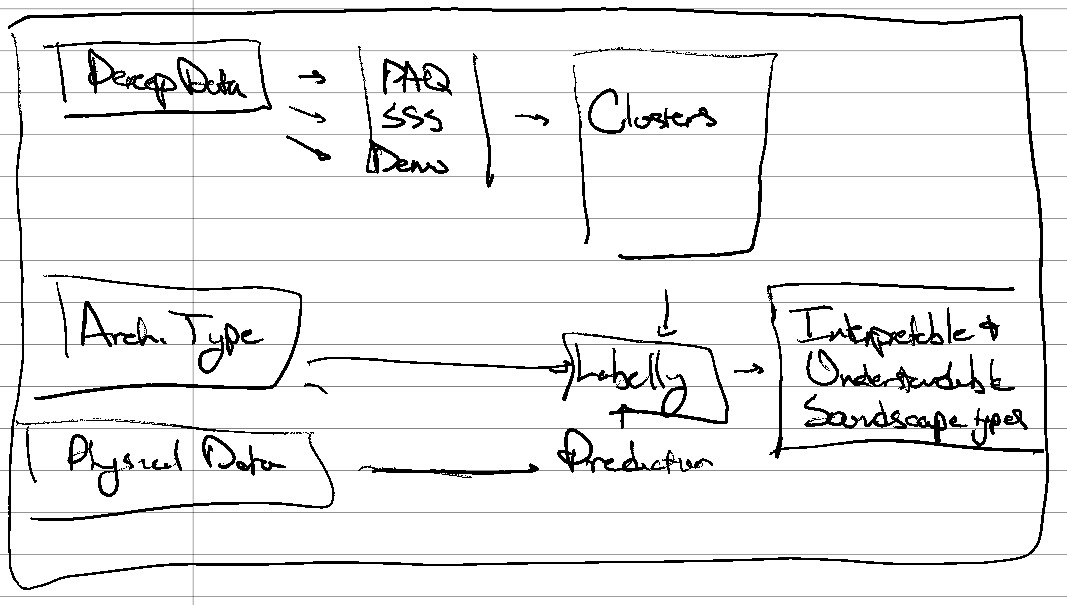
\includegraphics[width=\textwidth]{Figures/Remarkable clustering figure.jpg}
  \caption{Draft figure of a clustering approach}\label{fig:clusterModel}
\end{figure}

\draft{Issue with this approach to expand on: Limitations of starting dataset - impossible to know if we've identified all possible classes. Highly dependent on the primary dataset, the identified clusters cannot extend beyond what was already present.}